%% Marcas de dificultad
\providecommand{\facil}{\textcolor{bbe}{$\bigstar$}}
\providecommand{\medio}{\textcolor{bbe}{$\bigstar\bigstar$}}
\providecommand{\dificil}{\textcolor{bbe}{$\bigstar\bigstar\bigstar$}}

Esta secci\'on re\'une problemas para practicar todo lo visto en el cap\'itulo. Est\'a organizada en bloques que siguen el orden de las secciones, seguidos de un bloque de problemas mixtos (donde el m\'etodo no est\'a indicado), un bloque de aplicaciones y algunas actividades visuales. Al final encontrar\'a las respuestas de todos los problemas.

Cada problema lleva una marca de dificultad:
\begin{center}
\renewcommand{\arraystretch}{1.4}
\begin{tabular}{cl}
\facil & Aplicaci\'on directa del m\'etodo. \\
\medio & Requiere alg\'un paso adicional o una integral m\'as elaborada. \\
\dificil & Desaf\'io: requiere combinar ideas o un truco adicional. \\
\end{tabular}
\end{center}

Una sugerencia para estudiar: resuelva primero todos los problemas \facil\ de un bloque, luego al menos dos o tres \medio, y deje los \dificil\ para cuando domine el m\'etodo. Antes de mirar la respuesta, verifique su soluci\'on reemplaz\'andola en la ecuaci\'on: es la mejor forma de detectar errores.

\subsection*{\textquestiondown Qu\'e m\'etodo uso?}

En una prueba, el m\'etodo no viene indicado. El siguiente esquema resume las decisiones que hay que tomar frente a una ecuaci\'on lineal de segundo orden $a(x)y''+b(x)y'+c(x)y=f(x)$.

\begin{figure}[h!]
    \centering
    \begin{tikzpicture}[
        pregunta/.style={draw=bbeamber, fill=bbeamber!18, rounded corners=6pt, text width=2.8cm, align=center, minimum height=1.2cm, font=\footnotesize, text=black},
        accion/.style={draw=bbe, fill=bbe!8, rounded corners=2pt, text width=2.8cm, align=center, minimum height=1.2cm, font=\footnotesize, text=black},
        flecha/.style={->, thick, draw=bbe},
        si/.style={font=\footnotesize\bfseries, text=bbegreen, fill=white, inner sep=1pt},
        no/.style={font=\footnotesize\bfseries, text=bbered, fill=white, inner sep=1pt}
    ]
        \node[pregunta, text width=3.4cm] (q1) at (0.6,0) {\textquestiondown Los coeficientes $a,b,c$ son constantes?};
        \node[accion] (a1) at (-4,-2.2) {Resolver la homog\'enea con la ecuaci\'on auxiliar};
        \node[pregunta] (q3) at (3.4,-2.2) {\textquestiondown Es de Cauchy-Euler?\\ $x^2y''+a_1xy'+a_2y$};
        \node[pregunta] (q2) at (-4,-4.6) {\textquestiondown $f$ es polinomio, $e^{rx}$, seno, coseno, o sumas y productos de ellos?};
        \node[accion] (a4) at (1.0,-4.6) {Probar $y=x^r$ (o $x=e^z$). Para $y_p$: variaci\'on de par\'ametros o trabajar en $z$};
        \node[pregunta] (q4) at (5.8,-4.6) {\textquestiondown Conoce una soluci\'on $y_1$ de la homog\'enea?};
        \node[accion] (a2) at (-5.5,-7.4) {\textbf{Coeficientes indeterminados}\\ (revisar si hace falta el factor $x^s$)};
        \node[accion] (a3) at (-2.4,-7.4) {\textbf{Variaci\'on de par\'ametros}};
        \node[accion] (a5) at (4.2,-7.4) {\textbf{Reducci\'on de orden}\\ (entrega $y_2$ e $y_p$)};
        \node[accion] (a6) at (7.25,-7.4) {Buscar $y_1$ por inspecci\'on: $x^r$, $e^{rx}$, polinomios};
        \draw[flecha] (q1) -| node[si, pos=0.25] {S\'i} (a1);
        \draw[flecha] (q1) -| node[no, pos=0.25] {No} (q3);
        \draw[flecha] (a1) -- (q2);
        \draw[flecha] (q2) -| node[si, pos=0.3] {S\'i} (a2);
        \draw[flecha] (q2) -| node[no, pos=0.3] {No} (a3);
        \draw[flecha] (q3) -| node[si, pos=0.3] {S\'i} (a4);
        \draw[flecha] (q3) -| node[no, pos=0.3] {No} (q4);
        \draw[flecha] (q4) -| node[si, pos=0.3] {S\'i} (a5);
        \draw[flecha] (q4) -| node[no, pos=0.3] {No} (a6);
    \end{tikzpicture}
    \caption{Esquema de decisi\'on para elegir un m\'etodo. Recuerde que, si $f$ es una suma, el principio de superposici\'on permite usar un m\'etodo distinto para cada t\'ermino.}
    \label{fig:que_metodo}
\end{figure}

%======================================================================
\subsection*{A. Ecuaciones homog\'eneas de coeficientes constantes}

\begin{enumerate}[label=\textbf{A\arabic*.}, leftmargin=*]
    \item \facil\ Encuentre la soluci\'on general de:
    \begin{enumerate}[label=\alph*)]
        \item $y''-5y'+6y=0$.
        \item $y''+6y'+9y=0$.
        \item $y''+4y'+13y=0$.
    \end{enumerate}
    \item \facil\ Resuelva el PVI $\;y''-y'-2y=0,\quad y(0)=2,\quad y'(0)=1$.
    \item \facil\ Resuelva el PVI $\;y''+2y'+5y=0,\quad y(0)=1,\quad y'(0)=1$.
    \item \medio\ Encuentre la soluci\'on general de $y'''-y''-4y'+4y=0$.\\
    \textit{Indicaci\'on:} factorice la ecuaci\'on auxiliar agrupando t\'erminos.
    \item \medio\ Calcule el Wronskiano de $y_1=e^{2x}$ e $y_2=xe^{2x}$ y concluya que son linealmente independientes en $\mathbb{R}$.
    \item \dificil\ \textquestiondown Para qu\'e valores de la constante $k$ todas las soluciones de $y''+ky'+4y=0$ oscilan (es decir, cambian de signo infinitas veces)?
\end{enumerate}

%======================================================================
\subsection*{B. Coeficientes indeterminados}

\begin{example}[Problema modelo]
    Encuentre la soluci\'on general de $y''-3y'+2y=e^x+x$.

    \textbf{Primer paso: la homog\'enea.} La ecuaci\'on auxiliar $r^2-3r+2=(r-1)(r-2)=0$ tiene ra\'ices $1$ y $2$, as\'i que $y_h=C_1e^x+C_2e^{2x}$. \emph{Siempre conviene hacer esto primero}, porque las ra\'ices deciden la forma de $y_p$.

    \textbf{Segundo paso: separar $f$.} Por superposici\'on tratamos cada t\'ermino por separado:
    \begin{itemize}
        \item Para $e^x$: como $r=1$ es ra\'iz simple, la forma $Ae^x$ \emph{no sirve} (es soluci\'on de la homog\'enea). Proponemos $Axe^x$. Reemplazando se obtiene $-Ae^x=e^x$, luego $A=-1$.
        \item Para $x$: como $r=0$ no es ra\'iz, proponemos $Bx+C$. Reemplazando, $-3B+2Bx+2C=x$, luego $B=\frac12$, $C=\frac34$.
    \end{itemize}

    \textbf{Resultado:} $y=C_1e^x+C_2e^{2x}-xe^x+\dfrac{x}{2}+\dfrac{3}{4}$.

    \textbf{Error com\'un:} proponer $Ae^x$ sin revisar las ra\'ices y llegar a la contradicci\'on $0=e^x$.
\end{example}

\begin{enumerate}[label=\textbf{B\arabic*.}, leftmargin=*]
    \item \facil\ Encuentre una soluci\'on particular de:
    \begin{enumerate}[label=\alph*)]
        \item $y''+3y'+2y=4x^2$.
        \item $y''-y=3e^{2x}$.
        \item $y''+4y=3\sin x$.
    \end{enumerate}
    \item \medio\ Encuentre una soluci\'on particular de:
    \begin{enumerate}[label=\alph*)]
        \item $y''+4y=\sin(2x)$.
        \item $y''-4y'+4y=6e^{2x}$.
        \item $y''+y'=2x+1$.
    \end{enumerate}
    \textit{Indicaci\'on:} en los tres casos hay coincidencia con la soluci\'on homog\'enea.
    \item \medio\ \textbf{Solo la forma.} Sin calcular los coeficientes, escriba la forma de la soluci\'on particular que propondr\'ia para:
    \begin{enumerate}[label=\alph*)]
        \item $y''-4y'+4y=x^2e^{2x}+\cos x$.
        \item $y''+9y=x\sin(3x)$.
        \item $y''-2y'+5y=e^{x}\cos(2x)$.
        \item $y''+y'=x^3+e^{-x}$.
    \end{enumerate}
    \item \medio\ Resuelva el PVI $\;y''-y=2x,\quad y(0)=0,\quad y'(0)=1$.
    \item \dificil\ Encuentre una soluci\'on particular de $y''+y=x\cos x$.
\end{enumerate}

%======================================================================
\subsection*{C. Variaci\'on de par\'ametros}

\begin{example}[Problema modelo]
    Encuentre una soluci\'on particular de $y''+4y'+4y=x^{-2}e^{-2x}$, $x>0$.

    \textbf{\textquestiondown Por qu\'e variaci\'on de par\'ametros?} El factor $x^{-2}$ no pertenece a una familia cerrada bajo derivaci\'on, as\'i que coeficientes indeterminados no sirve.

    \textbf{Desarrollo.} Ra\'iz doble $r=-2$: $y_1=e^{-2x}$, $y_2=xe^{-2x}$, $W=e^{-4x}$. Con $f=x^{-2}e^{-2x}$ (la ecuaci\'on ya est\'a en forma est\'andar):
    \[
    u'=-\dfrac{xe^{-2x}\cdot x^{-2}e^{-2x}}{e^{-4x}}=-\dfrac1x,\qquad v'=\dfrac{e^{-2x}\cdot x^{-2}e^{-2x}}{e^{-4x}}=\dfrac{1}{x^2},
    \]
    de donde $u=-\ln x$, $v=-\dfrac1x$, y $y_p=-e^{-2x}\ln x-e^{-2x}$.

    \textbf{Simplificaci\'on:} el t\'ermino $-e^{-2x}$ es soluci\'on de la homog\'enea, as\'i que podemos eliminarlo: $y_p=-e^{-2x}\ln x$. \emph{Su respuesta puede diferir de la del libro en un t\'ermino de este tipo, y ambas son correctas.}
\end{example}

\begin{enumerate}[label=\textbf{C\arabic*.}, leftmargin=*]
    \item \facil\ $y''-4y'+5y=e^{2x}\tan x,\quad 0<x<\pi/2$.
    \item \facil\ $y''-6y'+9y=4e^{3x}\ln x,\quad x>0$.
    \item \facil\ $y''+2y'+y=\dfrac{e^{-x}}{\sqrt{4-x^2}},\quad |x|<2$.
    \item \medio\ \begin{enumerate}[label=\alph*)]
        \item $y''+6y'+9y=\dfrac{2e^{-3x}}{x^2+1}$.
        \item Generalice: $y''-2my'+m^2y=\dfrac{e^{mx}}{1+x^2}$, con $m$ constante. \textquestiondown Qu\'e obtiene para $m=5$?
    \end{enumerate}
    \item \medio\ $y''-4y=\dfrac{8}{e^{2x}+1}$.
    \item \medio\ $y''+9y=18\sec^3(3x),\quad |x|<\pi/6$.
    \item \medio\ $y''-2y'+y=4e^xx^{-3}\ln x,\quad x>0$.
    \item \medio\ $y''-6y'+13y=4e^{3x}\sec^2(2x),\quad |x|<\pi/4$.
    \item \dificil\ $y''+2y'+17y=\dfrac{64e^{-x}}{3+\sin^2(4x)}$.\\
    \textit{Indicaci\'on:} para una de las integrales escriba $3+\sin^2(4x)=4-\cos^2(4x)$.
    \item \dificil\ $y''+9y=\dfrac{36}{4-\cos^2(3x)}$.
\end{enumerate}

\noindent\textbf{Combinando m\'etodos.} En los siguientes problemas, use coeficientes indeterminados para una parte de $f$ y variaci\'on de par\'ametros para la otra.

\begin{enumerate}[label=\textbf{C\arabic*.}, leftmargin=*, resume]
    \item \medio\ $y''+y=\sec x+4e^x,\quad |x|<\pi/2$.
    \item \medio\ $y''+y=\csc x+2x^2+5x+1,\quad 0<x<\pi$.
    \item \medio\ $y''+4y'+4y=15e^{-2x}\ln x+25\cos x,\quad x>0$.
    \item \medio\ $y''+4y'+4y=\dfrac{4e^{-2x}}{1+x^2}+2x^2-1$.
\end{enumerate}

\noindent\textbf{Ecuaciones de tercer orden.} \textit{Indicaci\'on para C15 a C17:} si la ecuaci\'on auxiliar es $(r-r_0)^3=0$, la sustituci\'on $y=e^{r_0x}v$ transforma la ecuaci\'on en $v'''=e^{-r_0x}f(x)$, que se resuelve integrando tres veces.

\begin{enumerate}[label=\textbf{C\arabic*.}, leftmargin=*, resume]
    \item \dificil\ $y'''-6y''+12y'-8y=36e^{2x}\ln x,\quad x>0$.
    \item \dificil\ $y'''-3y''+3y'-y=2x^{-2}e^x,\quad x>0$.
    \item \dificil\ $y'''+3y''+3y'+y=\dfrac{2e^{-x}}{1+x^2}$.
\end{enumerate}

%======================================================================
\subsection*{D. Reducci\'on de orden y f\'ormula de Abel}

\begin{example}[Problema modelo]
    Sabiendo que $y_1=e^x$ es soluci\'on de $xy''+(1-2x)y'+(x-1)y=0$, $x>0$, encuentre la soluci\'on general.

    \textbf{Primer paso: forma est\'andar.} Dividiendo por $x$: $y''+\left(\dfrac1x-2\right)y'+\dfrac{x-1}{x}y=0$, as\'i que $P(x)=\dfrac1x-2$.

    \textbf{Segundo paso: Abel.} $-\int P\,dx=-\ln x+2x$, luego $e^{-\int P\,dx}=\dfrac{e^{2x}}{x}$.

    \textbf{Tercer paso: integrar.}
    \[
    y_2=e^x\int\dfrac{e^{2x}/x}{e^{2x}}\,dx=e^x\int\dfrac{dx}{x}=e^x\ln x.
    \]
    \textbf{Resultado:} $y=e^x\left(C_1+C_2\ln x\right)$.

    \textbf{Error com\'un:} usar $P(x)=1-2x$ (el coeficiente sin dividir por $x$).
\end{example}

\noindent En los siguientes problemas se conoce una soluci\'on $y_1$ de la ecuaci\'on homog\'enea. Use reducci\'on de orden para encontrar la soluci\'on general.

\begin{enumerate}[label=\textbf{D\arabic*.}, leftmargin=*]
    \item \facil\ $x^2y''-2xy'+(x^2+2)y=0,\quad x>0,\quad y_1=x\sin x$.
    \item \facil\ $y''-x^{-1}y'+4x^2y=0,\quad x>0,\quad y_1=\sin(x^2)$.
    \item \medio\ $(1-x^2)y''-2xy'+2y=0,\quad -1<x<1,\quad y_1=x$.\\
    \textit{Nota:} esta es la \textbf{ecuaci\'on de Legendre} de orden $1$, que aparece al estudiar problemas con simetr\'ia esf\'erica, como el potencial el\'ectrico alrededor de una esfera.
    \item \medio\ $4x^2y''+4xy'+(4x^2-1)y=0,\quad x>0,\quad y_1=x^{-1/2}\sin x$.\\
    \textit{Nota:} esta es la \textbf{ecuaci\'on de Bessel} de orden $\frac12$, que aparece al estudiar vibraciones de membranas circulares, como un tambor.
    \item \facil\ $y''-6y'+9y=15e^{3x}\sqrt{x},\quad x>0,\quad y_1=e^{3x}$.
    \item \facil\ $y''-4y'+4y=4e^{2x}\ln x,\quad x>0,\quad y_1=e^{2x}$.
    \item \medio\ $4x^2y''+y=\sqrt{x}\ln x,\quad x>0,\quad y_1=x^{1/2}$.
    \item \facil\ $y''+y=\csc x,\quad 0<x<\pi,\quad y_1=\sin x$.
    \item \medio\ $xy''-(2x+1)y'+2y=8x^2e^{2x},\quad x>0,\quad y_1=e^{2x}$.
    \item \facil\ $x^2y''-3xy'+4y=8x^4,\quad x>0,\quad y_1=x^2$.
    \item \medio\ \textbf{Abel sin resolver.} Sean $y_1,y_2$ dos soluciones de la ecuaci\'on de Legendre del problema D3 con $W[y_1,y_2](0)=1$. Sin conocer $y_1$ ni $y_2$, calcule $W[y_1,y_2](x)$ para $-1<x<1$.
    \item \dificil\ \textquestiondown Pueden $y_1=x$ e $y_2=\sin x$ ser ambas soluciones, en el intervalo $(-1,1)$, de una ecuaci\'on $y''+P(x)y'+Q(x)y=0$ con $P,Q$ continuas? Justifique usando la f\'ormula de Abel.\\
    \textit{Indicaci\'on:} calcule $W[y_1,y_2]$ y eval\'uelo en $x=0$.
\end{enumerate}

%======================================================================
\subsection*{E. Ecuaciones de Cauchy-Euler}

\noindent En todos los problemas de este bloque se considera $x>0$, salvo que se indique otra cosa.

\begin{example}[Problema modelo]
    Resuelva $x^2y''+xy'+9y=9\ln x$.

    \textbf{Homog\'enea.} La ecuaci\'on indicial es $r(r-1)+r+9=r^2+9=0$, con ra\'ices $\pm3i$ ($\alpha=0$, $\beta=3$). Luego $y_h=C_1\cos(3\ln x)+C_2\sin(3\ln x)$.

    \textbf{Particular, trabajando en $z$.} Con $x=e^z$ la ecuaci\'on se transforma en $\ddot y+9y=9z$, una ecuaci\'on de coeficientes constantes con lado derecho polinomial. Proponiendo $y_p=Az+B$ se obtiene $9Az+9B=9z$, as\'i que $y_p=z=\ln x$.

    \textbf{Resultado:} $y=C_1\cos(3\ln x)+C_2\sin(3\ln x)+\ln x$.

    \textbf{Idea clave:} en la variable $z$, el lado derecho $\ln x=z$ es un polinomio, y podemos usar coeficientes indeterminados. Esto funciona siempre que $f$ sea de la forma $x^a(\ln x)^k$, $x^a\cos(b\ln x)$, etc.
\end{example}

\begin{enumerate}[label=\textbf{E\arabic*.}, leftmargin=*]
    \item \facil\ Encuentre la soluci\'on general de:
    \begin{enumerate}[label=\alph*)]
        \item $x^2y''+xy'-4y=0$.
        \item $x^2y''-xy'+y=0$.
    \end{enumerate}
    \item \facil\ $x^2y''+4xy'+2y=4\ln x$.
    \item \medio\ $x^2y''-4xy'+6y=x^4\sin x$.
    \item \medio\ $x^2y''+6xy'+6y=4e^{2x}$.
    \item \medio\ $x^2y''-3xy'+4y=\dfrac{x^2}{\ln x},\quad x>1$.
    \item \facil\ $x^2y''+4xy'+2y=\cos x$.\\
    \textit{Indicaci\'on:} compruebe que $x^2y''+4xy'+2y=\left(x^2y\right)''$. \textquestiondown Puede usar esta observaci\'on tambi\'en en E2?
    \item \medio\ $x^2y''-xy'+5y=8x(\ln x)^2$.
    \item \dificil\ $x^2y''-(2m-1)xy'+m^2y=x^m(\ln x)^k$, donde $m,k$ son constantes y $x>1$.\\
    Discuta por separado los casos $k=-1$ y $k=-2$. \textquestiondown Qu\'e problema anterior corresponde a $m=2$, $k=-1$?
\end{enumerate}

\begin{remark}[Forma amplitud-fase]
    Una combinaci\'on $C_1\cos\theta+C_2\sin\theta$ siempre se puede escribir como una sola funci\'on coseno:
    \[
    C_1\cos\theta+C_2\sin\theta=A\cos(\theta-\varphi),
    \]
    donde
    \[
    A=\sqrt{C_1^2+C_2^2},\qquad \cos\varphi=\dfrac{C_1}{A},\qquad \sin\varphi=\dfrac{C_2}{A}.
    \]
    Esto se comprueba expandiendo $A\cos(\theta-\varphi)=A\cos\varphi\cos\theta+A\sin\varphi\sin\theta$. La forma amplitud-fase es muy \'util para interpretar soluciones oscilantes: $A$ es la amplitud y $\varphi$ el desfase.
\end{remark}

\begin{enumerate}[label=\textbf{E\arabic*.}, leftmargin=*, resume]
    \item \medio\ Resuelva el PVI
    \[
    x^2y''-xy'+5y=0,\qquad y(1)=\sqrt2,\qquad y'(1)=3\sqrt2,
    \]
    y pruebe que la soluci\'on se puede escribir como $y(x)=2x\cos\left(2\ln x-\dfrac{\pi}{4}\right)$.
    \item \medio\ Resuelva el PVI
    \[
    t^2\dfrac{d^2y}{dt^2}+t\dfrac{dy}{dt}+25y=0,\qquad y(1)=\dfrac{3\sqrt3}{2},\qquad y'(1)=\dfrac{15}{2},
    \]
    y muestre que la soluci\'on se puede escribir como $y(t)=3\cos\left(5\ln t-\dfrac{\pi}{6}\right)$. \textquestiondown Cu\'al es la amplitud de la oscilaci\'on? \textquestiondown Depende de $t$?
\end{enumerate}

%======================================================================
\subsection*{F. Problemas mixtos y preguntas conceptuales}

\begin{example}[Problema modelo: elegir el m\'etodo]
    Sin resolver, decida qu\'e m\'etodo usar\'ia para cada ecuaci\'on y justifique.
    \begin{enumerate}[label=\alph*)]
        \item $y''-y=xe^x$. \textbf{Coeficientes indeterminados:} coeficientes constantes y $f$ es polinomio por exponencial. Como $r=1$ es ra\'iz simple, la forma es $x(Ax+B)e^x$.
        \item $y''+y=\sec x$. \textbf{Variaci\'on de par\'ametros:} $\sec x$ no est\'a en la lista de funciones admitidas.
        \item $x^2y''+xy'-y=x$. \textbf{Cauchy-Euler:} la homog\'enea se resuelve con $x^r$ ($r=\pm1$). Para $y_p$, en la variable $z$ el lado derecho es $e^z$, y como $r=1$ es ra\'iz, se propone $Aze^z$; se obtiene $y_p=\frac12x\ln x$.
    \end{enumerate}
\end{example}

\begin{enumerate}[label=\textbf{F\arabic*.}, leftmargin=*]
    \item \medio\ Resuelva por el m\'etodo que le parezca m\'as conveniente:
    \begin{enumerate}[label=\alph*)]
        \item $y''+4y=\sin(2x)$.
        \item $y''+4y=\csc(2x),\quad 0<x<\pi/2$.
        \item $x^2y''-2y=x^3,\quad x>0$.
        \item $y''-2y'+y=\dfrac{e^x}{x},\quad x>0$.
        \item $y''+y'-2y=3e^x$.
    \end{enumerate}
    Compare a) con b): tienen el mismo lado izquierdo, \textquestiondown por qu\'e requieren m\'etodos distintos?
    \item \facil\ \textbf{Verdadero o falso.} Justifique cada respuesta.
    \begin{enumerate}[label=\alph*)]
        \item Si $y_1,y_2$ son soluciones de $y''+P(x)y'+Q(x)y=0$ con $P,Q$ continuas, y su Wronskiano se anula en un punto $x_0$, entonces $y_1$ e $y_2$ son linealmente dependientes.
        \item Una soluci\'on particular de $y''+y=\tan x$ se puede obtener por coeficientes indeterminados.
        \item Si $r=2$ es ra\'iz doble de la ecuaci\'on auxiliar, entonces la forma de $y_p$ para $f=e^{2x}$ es $Axe^{2x}$.
        \item La suma de dos soluciones de $y''+y=x$ es tambi\'en soluci\'on de $y''+y=x$.
        \item La ecuaci\'on $x^2y''+y=0$ tiene soluciones que oscilan en $x>0$.
    \end{enumerate}
    \item \medio\ \textbf{Problema inverso.} Encuentre una ecuaci\'on diferencial cuya soluci\'on general sea la indicada.
    \begin{enumerate}[label=\alph*)]
        \item $y=e^{-x}\left(C_1\cos 2x+C_2\sin 2x\right)$, con coeficientes constantes.
        \item $y=C_1e^{3x}+C_2xe^{3x}+x$, con coeficientes constantes.
        \item $y=C_1x+C_2x^3$, $x>0$, de tipo Cauchy-Euler.
    \end{enumerate}
    \item \facil\ Explique con sus palabras por qu\'e el m\'etodo de coeficientes indeterminados no permite resolver el problema C1, y por qu\'e variaci\'on de par\'ametros s\'i.
\end{enumerate}

%======================================================================
\subsection*{G. Aplicaciones}

\begin{enumerate}[label=\textbf{G\arabic*.}, leftmargin=*]
    \item \medio\ \textbf{Tipos de amortiguaci\'on.} Una masa de $1\,\mathrm{kg}$ unida a un resorte de constante $k=4\,\mathrm{N/m}$ se mueve en un medio con coeficiente de amortiguaci\'on $b\geq0$, de modo que su posici\'on satisface $y''+by'+4y=0$.
    \begin{enumerate}[label=\alph*)]
        \item Determine para qu\'e valores de $b$ el movimiento es \emph{subamortiguado} (ra\'ices complejas: la masa oscila), \emph{cr\'iticamente amortiguado} (ra\'iz doble) o \emph{sobreamortiguado} (ra\'ices reales distintas).
        \item Resuelva el caso cr\'itico con $y(0)=1$, $y'(0)=0$.
        \item Sin hacer c\'alculos, \textquestiondown qu\'e cree que ocurre con la soluci\'on cuando $t\to\infty$ en los tres casos? \textquestiondown Por qu\'e los amortiguadores de un auto se dise\~nan cerca del caso cr\'itico?
    \end{enumerate}
    \item \medio\ \textbf{Pulsaciones y resonancia.} Un sistema masa-resorte sin amortiguaci\'on, inicialmente en reposo en su posici\'on de equilibrio, es sometido a una fuerza externa peri\'odica:
    \[
    y''+9y=\cos(\omega t),\qquad y(0)=0,\qquad y'(0)=0.
    \]
    \begin{enumerate}[label=\alph*)]
        \item Resuelva el PVI para $\omega\neq3$.
        \item Resuelva el PVI para $\omega=3$.
        \item La Figura~\ref{fig:pulsaciones} muestra la soluci\'on para $\omega=2{,}8$ y para $\omega=3$. Describa la diferencia entre ambos comportamientos. \textquestiondown Qu\'e ocurre con la soluci\'on de a) cuando $\omega\to3$?
    \end{enumerate}
    \item \medio\ \textbf{Circuito RLC.} La carga $q(t)$ en un circuito con una inductancia $L$, una resistencia $R$, un condensador de capacidad $C$ y una fuente de voltaje $E(t)$ satisface
    \[
    L\,q''+R\,q'+\dfrac{1}{C}\,q=E(t).
    \]
    Esta es exactamente la ecuaci\'on de un sistema masa-resorte, con la siguiente analog\'ia:
    \begin{center}
    \renewcommand{\arraystretch}{1.3}
    \begin{tabular}{|c|c|c|c|c|}
    \hline
    Masa $m$ & Amortiguaci\'on $b$ & Resorte $k$ & Fuerza $f(t)$ & Posici\'on $y$\\ \hline
    Inductancia $L$ & Resistencia $R$ & $1/C$ & Voltaje $E(t)$ & Carga $q$\\ \hline
    \end{tabular}
    \end{center}
    Considere $L=1$, $R=2$, $C=\frac15$ y $E(t)=10\cos t$, con $q(0)=0$, $q'(0)=0$.
    \begin{enumerate}[label=\alph*)]
        \item Encuentre $q(t)$.
        \item Identifique la parte \emph{transitoria} (la que tiende a cero) y la parte \emph{estacionaria} de la soluci\'on.
        \item Escriba la parte estacionaria en forma amplitud-fase y determine su amplitud.
    \end{enumerate}
\end{enumerate}

\begin{figure}[h!]
    \centering
    \begin{subfigure}[b]{0.48\textwidth}
        \centering
        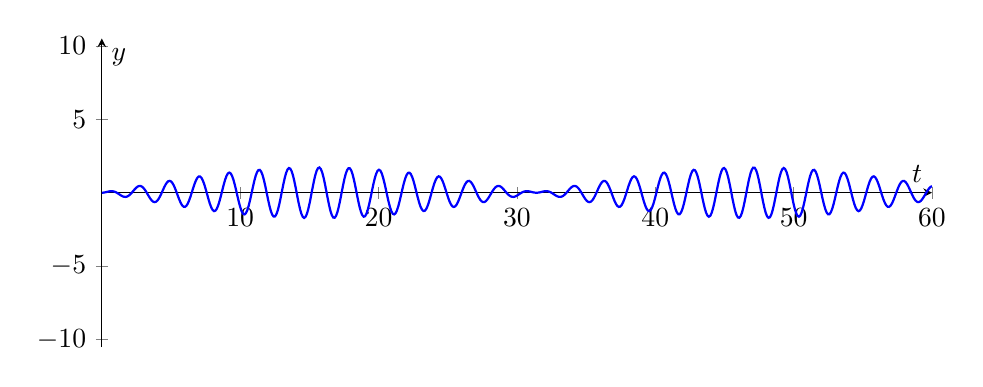
\begin{tikzpicture}
            \begin{axis}[
                axis lines = middle,
                xlabel = $t$, ylabel = {$y$},
                xmin=0, xmax=60, ymin=-10.5, ymax=10.5,
                width=\textwidth, height=5.5cm
            ]
            \addplot[domain=0:60, samples=600, blue, thick] {(cos(deg(2.8*x)) - cos(deg(3*x)))/1.16};
            \end{axis}
        \end{tikzpicture}
        \caption{$\omega=2{,}8$}
    \end{subfigure}
    \hfill
    \begin{subfigure}[b]{0.48\textwidth}
        \centering
        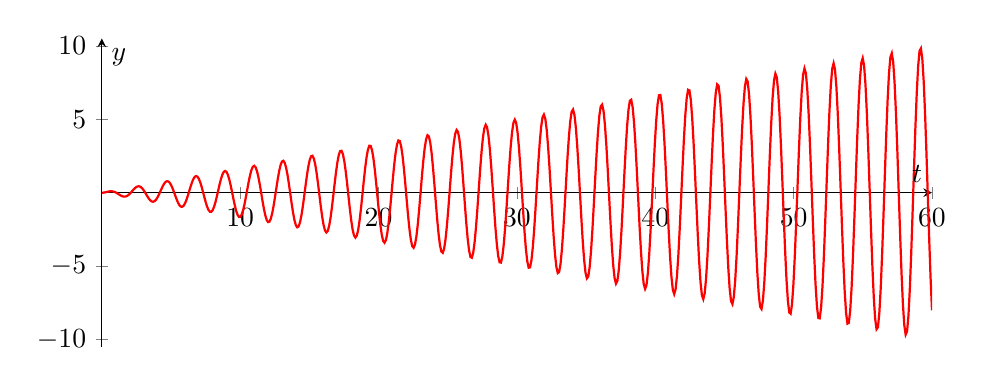
\begin{tikzpicture}
            \begin{axis}[
                axis lines = middle,
                xlabel = $t$, ylabel = {$y$},
                xmin=0, xmax=60, ymin=-10.5, ymax=10.5,
                width=\textwidth, height=5.5cm
            ]
            \addplot[domain=0:60, samples=600, red, thick] {x*sin(deg(3*x))/6};
            \end{axis}
        \end{tikzpicture}
        \caption{$\omega=3$}
    \end{subfigure}
    \caption{Soluciones del problema G2 para dos frecuencias de la fuerza externa.}
    \label{fig:pulsaciones}
\end{figure}

%======================================================================
\subsection*{Actividades}

\begin{activity}[Emparejar gr\'aficos con ecuaciones]
    Los siguientes gr\'aficos corresponden a las soluciones de los cuatro PVI de la lista, pero en otro orden. Sin resolver las ecuaciones, determine qu\'e gr\'afico corresponde a cada PVI y justifique su elecci\'on usando las ra\'ices de la ecuaci\'on auxiliar o indicial.
    \begin{enumerate}[label=\arabic*.]
        \item $y''+2y'+y=0,\qquad y(0)=1,\ y'(0)=0$.
        \item $y''+0{,}4\,y'+4y=0,\qquad y(0)=1,\ y'(0)=0$.
        \item $y''+4y=\cos(2t),\qquad y(0)=0,\ y'(0)=0$.
        \item $t^2y''+ty'+16y=0,\qquad y(1)=1,\ y'(1)=0,\quad t>0$.
    \end{enumerate}
    \textit{Pistas:} \textquestiondown qu\'e soluciones oscilan? \textquestiondown Cu\'al tiene amplitud creciente? \textquestiondown En cu\'al las oscilaciones no est\'an igualmente espaciadas?
\end{activity}

\begin{figure}[h!]
    \centering
    \begin{subfigure}[b]{0.48\textwidth}
        \centering
        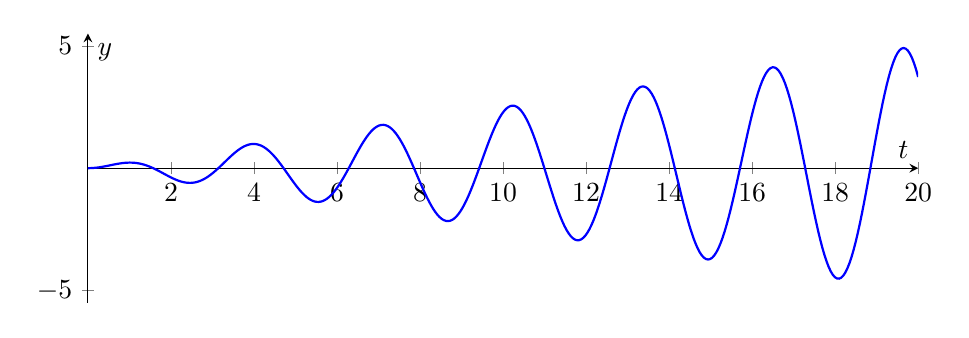
\begin{tikzpicture}
            \begin{axis}[
                axis lines = middle, xlabel = $t$, ylabel = {$y$},
                xmin=0, xmax=20, ymin=-5.5, ymax=5.5,
                width=\textwidth, height=5cm
            ]
            \addplot[domain=0:20, samples=400, blue, thick] {x*sin(deg(2*x))/4};
            \end{axis}
        \end{tikzpicture}
        \caption{Gr\'afico A}
    \end{subfigure}
    \hfill
    \begin{subfigure}[b]{0.48\textwidth}
        \centering
        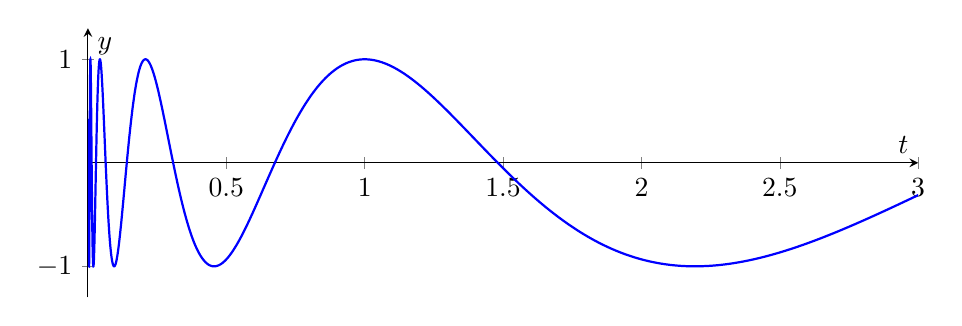
\begin{tikzpicture}
            \begin{axis}[
                axis lines = middle, xlabel = $t$, ylabel = {$y$},
                xmin=0, xmax=3, ymin=-1.3, ymax=1.3,
                width=\textwidth, height=5cm
            ]
            \addplot[domain=-6:1.1, samples=800, blue, thick] ({exp(x)},{cos(deg(4*x))});
            \end{axis}
        \end{tikzpicture}
        \caption{Gr\'afico B}
    \end{subfigure}

    \vspace{0.3cm}
    \begin{subfigure}[b]{0.48\textwidth}
        \centering
        \begin{tikzpicture}
            \begin{axis}[
                axis lines = middle, xlabel = $t$, ylabel = {$y$},
                xmin=0, xmax=8, ymin=-0.2, ymax=1.2,
                width=\textwidth, height=5cm
            ]
            \addplot[domain=0:8, samples=200, blue, thick] {(1+x)*exp(-x)};
            \end{axis}
        \end{tikzpicture}
        \caption{Gr\'afico C}
    \end{subfigure}
    \hfill
    \begin{subfigure}[b]{0.48\textwidth}
        \centering
        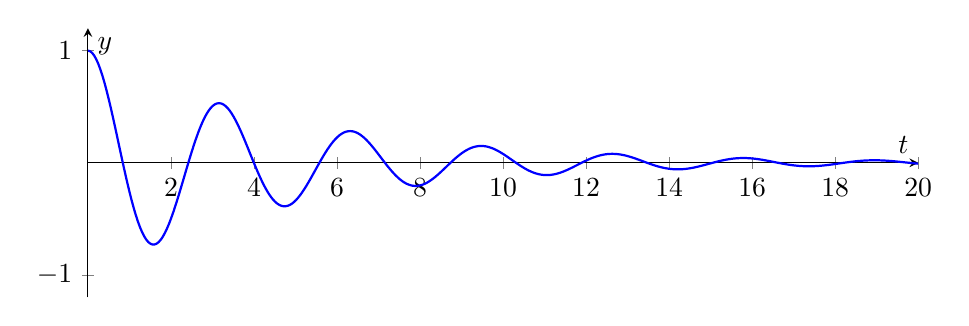
\begin{tikzpicture}
            \begin{axis}[
                axis lines = middle, xlabel = $t$, ylabel = {$y$},
                xmin=0, xmax=20, ymin=-1.2, ymax=1.2,
                width=\textwidth, height=5cm
            ]
            \addplot[domain=0:20, samples=400, blue, thick] {exp(-0.2*x)*(cos(deg(1.98997*x)) + (0.2/1.98997)*sin(deg(1.98997*x)))};
            \end{axis}
        \end{tikzpicture}
        \caption{Gr\'afico D}
    \end{subfigure}
    \caption{Gr\'aficos para la actividad de emparejamiento.}
    \label{fig:emparejar}
\end{figure}

\begin{activity}[Exploraci\'on con software]
    Use GeoGebra o Desmos (ambos gratuitos y disponibles en l\'inea) para explorar la familia de soluciones del problema E10,
    \[
    y(t)=C_1\cos(5\ln t)+C_2\sin(5\ln t),\qquad t>0.
    \]
    \begin{enumerate}[label=\alph*)]
        \item Defina dos deslizadores para $C_1$ y $C_2$ y grafique $y(t)$.
        \item Mueva los deslizadores. \textquestiondown Qu\'e cambia en el gr\'afico? \textquestiondown Qu\'e se mantiene? Relacione sus observaciones con la forma amplitud-fase $A\cos(5\ln t-\varphi)$.
        \item Grafique la misma funci\'on en funci\'on de $z=\ln t$, es decir, $y=C_1\cos(5z)+C_2\sin(5z)$. \textquestiondown Qu\'e diferencia observa? Relacione con el cambio de variable $t=e^z$.
        \item Encuentre $C_1$ y $C_2$ para que la gr\'afica pase por el punto $(1,2)$ con tangente horizontal. Verifique su resultado resolviendo el PVI correspondiente.
    \end{enumerate}
\end{activity}

%======================================================================
\newpage
\subsection*{Respuestas}

{\small\sloppy
\noindent En las respuestas, $C_1,C_2,C_3$ denotan constantes arbitrarias. Recuerde que una soluci\'on particular puede diferir de la indicada en una soluci\'on de la ecuaci\'on homog\'enea.

\paragraph{Bloque A.}
\begin{enumerate}[label=\textbf{A\arabic*.}, leftmargin=*]
    \item a) $y=C_1e^{2x}+C_2e^{3x}$. \quad b) $y=(C_1+C_2x)e^{-3x}$. \quad c) $y=e^{-2x}\left(C_1\cos3x+C_2\sin3x\right)$.
    \item $y=e^{2x}+e^{-x}$.
    \item $y=e^{-x}\left(\cos2x+\sin2x\right)$.
    \item $(r-1)(r^2-4)=0$, luego $y=C_1e^x+C_2e^{2x}+C_3e^{-2x}$.
    \item $W=e^{4x}\neq0$.
    \item Las soluciones oscilan cuando las ra\'ices son complejas: $k^2-16<0$, es decir, $-4<k<4$.
\end{enumerate}

\paragraph{Bloque B.}
\begin{enumerate}[label=\textbf{B\arabic*.}, leftmargin=*]
    \item a) $y_p=2x^2-6x+7$. \quad b) $y_p=e^{2x}$. \quad c) $y_p=\sin x$.
    \item a) $y_p=-\dfrac{x}{4}\cos 2x$. \quad b) $y_p=3x^2e^{2x}$. \quad c) $y_p=x^2-x$.
    \item a) $x^2\left(Ax^2+Bx+C\right)e^{2x}+D\cos x+E\sin x$. \quad b) $x\left[(Ax+B)\cos3x+(Cx+D)\sin3x\right]$.\\
    c) $xe^x\left(A\cos2x+B\sin2x\right)$. \quad d) $x\left(Ax^3+Bx^2+Cx+D\right)+Exe^{-x}$.
    \item $y=3\sinh x-2x=\dfrac32\left(e^x-e^{-x}\right)-2x$.
    \item $y_p=\dfrac{x}{4}\cos x+\dfrac{x^2}{4}\sin x$.
\end{enumerate}

\paragraph{Bloque C.} Se indica una soluci\'on particular.
\begin{enumerate}[label=\textbf{C\arabic*.}, leftmargin=*]
    \item $y_p=-e^{2x}\cos x\,\ln\left(\sec x+\tan x\right)$.
    \item $y_p=x^2e^{3x}\left(2\ln x-3\right)$.
    \item $y_p=e^{-x}\left(x\arcsin\dfrac{x}{2}+\sqrt{4-x^2}\right)$.
    \item a) $y_p=e^{-3x}\left(2x\arctan x-\ln\left(1+x^2\right)\right)$. \quad b) $y_p=e^{mx}\left(x\arctan x-\frac12\ln\left(1+x^2\right)\right)$; con $m=5$ se obtiene la soluci\'on de $y''-10y'+25y=\frac{e^{5x}}{1+x^2}$.
    \item $y_p=e^{2x}\ln\left(1+e^{-2x}\right)-e^{-2x}\ln\left(1+e^{2x}\right)-1$.
    \item $y_p=-\dfrac{\cos 6x}{\cos 3x}=2\sin3x\tan3x-\sec3x$.
    \item $y_p=\dfrac{e^x}{x}\left(2\ln x+3\right)$.
    \item $y_p=e^{3x}\left[\sin(2x)\ln\left(\sec2x+\tan2x\right)-1\right]$.
    \item $y_p=e^{-x}\left[\cos(4x)\ln\dfrac{2+\cos4x}{2-\cos4x}+\dfrac{4}{\sqrt3}\sin(4x)\arctan\dfrac{\sin4x}{\sqrt3}\right]$.
    \item $y_p=\cos(3x)\ln\dfrac{2+\cos3x}{2-\cos3x}+\dfrac{4}{\sqrt3}\sin(3x)\arctan\dfrac{\sin3x}{\sqrt3}$.
    \item $y_p=x\sin x+\cos x\ln(\cos x)+2e^x$.
    \item $y_p=-x\cos x+\sin x\ln(\sin x)+2x^2+5x-3$.
    \item $y_p=\dfrac{15}{4}x^2e^{-2x}\left(2\ln x-3\right)+3\cos x+4\sin x$.
    \item $y_p=e^{-2x}\left(4x\arctan x-2\ln\left(1+x^2\right)\right)+\dfrac{(x-1)^2}{2}$.
    \item $y_p=x^3e^{2x}\left(6\ln x-11\right)$.
    \item $y_p=-2xe^x\ln x$.
    \item $y_p=e^{-x}\left[\left(x^2-1\right)\arctan x-x\ln\left(1+x^2\right)\right]$.
\end{enumerate}

\paragraph{Bloque D.}
\begin{enumerate}[label=\textbf{D\arabic*.}, leftmargin=*]
    \item $y=C_1x\sin x+C_2x\cos x$.
    \item $y=C_1\sin\left(x^2\right)+C_2\cos\left(x^2\right)$.
    \item $y=C_1x+C_2\left(\dfrac{x}{2}\ln\dfrac{1+x}{1-x}-1\right)$.
    \item $y=x^{-1/2}\left(C_1\sin x+C_2\cos x\right)$.
    \item $y=e^{3x}\left(C_1+C_2x+4x^{5/2}\right)$.
    \item $y=e^{2x}\left(C_1+C_2x+2x^2\ln x-3x^2\right)$.
    \item $y=\sqrt{x}\left(C_1+C_2\ln x\right)+\dfrac{1}{24}\sqrt{x}\,(\ln x)^3$.
    \item $y=C_1\sin x+C_2\cos x-x\cos x+\sin x\ln(\sin x)$.
    \item $y_2=2x+1$ \ (salvo constante), \ $y=C_1e^{2x}+C_2(2x+1)+2x^2e^{2x}$.
    \item $y=C_1x^2+C_2x^2\ln x+2x^4$.
    \item $W[y_1,y_2](x)=\dfrac{1}{1-x^2}$.
    \item No. $W[x,\sin x]=x\cos x-\sin x$ se anula en $x=0$ pero no es id\'enticamente cero en $(-1,1)$, lo que contradice la f\'ormula de Abel.
\end{enumerate}

\paragraph{Bloque E.}
\begin{enumerate}[label=\textbf{E\arabic*.}, leftmargin=*]
    \item a) $y=C_1x^2+C_2x^{-2}$. \quad b) $y=x\left(C_1+C_2\ln x\right)$.
    \item $y=C_1x^{-1}+C_2x^{-2}+2\ln x-3$.
    \item $y=C_1x^2+C_2x^3-x^2\sin x$.
    \item $y=C_1x^{-2}+C_2x^{-3}+\dfrac{e^{2x}(x-1)}{x^3}$.
    \item $y=x^2\left(C_1+C_2\ln x\right)+x^2\ln x\,\ln(\ln x)$.
    \item $y=C_1x^{-1}+C_2x^{-2}-\dfrac{\cos x}{x^2}$. S\'i: en E2 se obtiene $\left(x^2y\right)''=4\ln x$.
    \item $y=x\left(C_1\cos(2\ln x)+C_2\sin(2\ln x)\right)+x\left(2(\ln x)^2-1\right)$.
    \item La ecuaci\'on indicial es $(r-m)^2=0$, as\'i que $y_h=x^m\left(C_1+C_2\ln x\right)$. Para $k\neq-1,-2$: $y_p=\dfrac{x^m(\ln x)^{k+2}}{(k+1)(k+2)}$. Para $k=-1$: $y_p=x^m\ln x\,\ln(\ln x)$. Para $k=-2$: $y_p=-x^m\ln(\ln x)$. El caso $m=2$, $k=-1$ es el problema E5.
    \item $y=\sqrt2\,x\left(\cos(2\ln x)+\sin(2\ln x)\right)=2x\cos\left(2\ln x-\frac\pi4\right)$.
    \item $y=\frac{3\sqrt3}{2}\cos(5\ln t)+\frac32\sin(5\ln t)=3\cos\left(5\ln t-\frac\pi6\right)$. La amplitud es $3$ y no depende de $t$.
\end{enumerate}

\paragraph{Bloque F.}
\begin{enumerate}[label=\textbf{F\arabic*.}, leftmargin=*]
    \item a) $y=C_1\cos2x+C_2\sin2x-\dfrac{x}{4}\cos2x$ (coeficientes indeterminados, con resonancia).\\
    b) $y=C_1\cos2x+C_2\sin2x-\dfrac{x}{2}\cos2x+\dfrac14\sin(2x)\ln(\sin2x)$ (variaci\'on de par\'ametros).\\
    c) $y=C_1x^2+C_2x^{-1}+\dfrac{x^3}{4}$.\\ d) $y=e^x\left(C_1+C_2x\right)+xe^x\ln x$. \quad e) $y=C_1e^x+C_2e^{-2x}+xe^x$.\\
    El lado izquierdo es el mismo; lo que decide el m\'etodo es la funci\'on $f$: $\sin 2x$ est\'a en la familia admitida, $\csc 2x$ no.
    \item a) Verdadero: por la f\'ormula de Abel, si el Wronskiano se anula en un punto, es id\'enticamente cero. \quad b) Falso: $\tan x$ no es de un tipo admitido. \quad c) Falso: la forma es $Ax^2e^{2x}$. \quad d) Falso: la suma es soluci\'on de $y''+y=2x$.\\ e) Verdadero: la ecuaci\'on indicial $r^2-r+1=0$ tiene ra\'ices $\frac12\pm\frac{\sqrt3}{2}i$, y las soluciones son $\sqrt{x}\cos\left(\frac{\sqrt3}{2}\ln x\right)$ y $\sqrt{x}\sin\left(\frac{\sqrt3}{2}\ln x\right)$.
    \item a) $y''+2y'+5y=0$. \quad b) $y''-6y'+9y=9x-6$. \quad c) $x^2y''-3xy'+3y=0$.
    \item El lado derecho $e^{2x}\tan x$ contiene $\tan x$, cuyas derivadas generan funciones nuevas ($\sec^2x$, $\sec^2x\tan x$, \ldots), as\'i que no hay una forma finita que proponer. Variaci\'on de par\'ametros funciona para cualquier $f$ continua, porque solo requiere calcular integrales.
\end{enumerate}

\paragraph{Bloque G.}
\begin{enumerate}[label=\textbf{G\arabic*.}, leftmargin=*]
    \item a) Subamortiguado si $0\leq b<4$, cr\'itico si $b=4$, sobreamortiguado si $b>4$. \quad b) $y=(1+2t)e^{-2t}$.\\ c) En los tres casos $y\to0$ (la energ\'ia se disipa). El caso cr\'itico es el que vuelve al equilibrio m\'as r\'apido sin oscilar, lo que da una conducci\'on c\'omoda y estable.
    \item a) $y=\dfrac{\cos(\omega t)-\cos(3t)}{9-\omega^2}$. \quad b) $y=\dfrac{t}{6}\sin(3t)$. \quad c) Para $\omega=2{,}8$ la amplitud crece y decrece peri\'odicamente (\emph{pulsaciones}) sin superar un valor m\'aximo; en cambio, para $\omega=3$ la amplitud crece sin l\'imite (\emph{resonancia}). Cuando $\omega\to3$, la soluci\'on de a) tiende a la de b) (aplique la regla de L'H\^opital en $\omega$).
    \item a) $q(t)=e^{-t}\left(-2\cos2t-\frac32\sin2t\right)+2\cos t+\sin t$. \quad b) Transitoria: $e^{-t}\left(-2\cos2t-\frac32\sin2t\right)$; estacionaria: $2\cos t+\sin t$. \quad c) $2\cos t+\sin t=\sqrt5\cos(t-\varphi)$ con $\tan\varphi=\frac12$; la amplitud es $\sqrt5$.
\end{enumerate}

\paragraph{Actividad de emparejamiento.} 1 $\to$ C (ra\'iz doble: vuelve al equilibrio sin oscilar); 2 $\to$ D (ra\'ices complejas con parte real negativa: oscila con amplitud decreciente); 3 $\to$ A (resonancia: $y=\frac{t}{4}\sin 2t$, amplitud creciente); 4 $\to$ B (Cauchy-Euler: $y=\cos(4\ln t)$, oscilaciones que se acumulan cerca de $t=0$).

\paragraph{Actividad de exploraci\'on.} d) $C_1=2$, $C_2=0$, es decir, $y=2\cos(5\ln t)$.
}
